\chapter{高级SDN程序中循环结构的数据通路实现问题的研究} 
%\tableofcontents
%
%\section{摘要}
%%To achieve the offloading of complex computations to the network may require the remote access to state variables in stateful switches of the network. However, the remote access imposes new consistency issues among the accessing processes. In this paper, we first analyze the consistency issues in the remote access to state variables. We then present \system{}, a unified state variable access framework to achieve coexistence of multiple accesses with different consistency requirements. \system{} includes an event-based state variable access model to remove the complexities of handling the remote access. We demonstrate the expressiveness of \system{} and conduct an extensive evaluation to show the effectiveness.
%
%尽管高级SDN编程的发展提高了编程的灵活性,但由于现有的硬件限制,SDN程序中的循环(如,\codeword{while})还不能部署在数据通路中。 针对部署在流水线架构数据通路的SDN程序中的循环部分,本章提出用重复软件流水线(repeated software pipeline,RSP)变换来解决编译问题。该方法支持动态的循环条件,并在循环次数较大情况下依然有效。实验评估发现,在某些情况下,RSP的效率比循环展开方法快10倍。




\section{引言} 
\label{sec:intro}

高级SDN编程技术的发展在保持了编程模型的灵活性的同时,也降低了数据包处理的延时。主动式地将高级程序编译为数据通路正是一个代表性技术。基于由高级程序生成的数据通路,数据包无需再传给控制器等待处理。保持SDN程序的高级编程模型可以提高程序的可读性从而降低程序发生错误的风险。此外,编程模型的高度灵活性允许程序员用简单的语法,例如\codeword{if, else, while},描述复杂的逻辑。

然而,由于硬件条件的限制,复杂的逻辑很难部署到数据通路中,特别是在高级编程中非常有用的循环语句,在当前的数据通路体系结构(即多流表流水线)中却无法支持。因此,要在数据通路中部署循环部分的逻辑,必须在保持逻辑不变的情况下对它们进行转换。

一个简单的转换是基于黑盒模型。该模型将整个循环视为具有多个输入和输出的单个语句。然而,由黑盒方法生成的单语句结构不能利用数据通路中的多流表流水线。进而由于单流表中数据包匹配域的叉乘(cross-product),流表规则数量将大幅度增加~\cite{openflow1-3-1},当流表不能再接受新的流规则时会影响系统性能。

另一个转换是从编译器领域引出的循环展开(unroll)的方法。通过展开,循环将由一串的顺序语句代替。具体地说,编译器领域中的展开方法依赖于显式的循环索引,例如\codeword{for i in range(10)}中的\codeword{i}。并基于循环索引的值将循环展开为多个循环过程中的语句块。然后这些块连接在一起。但是循环展开方法是受限的。因为它只能支持循环次数明确的循环(即静态循环条件),例如\codeword{for i in range(10)} 。更通用的循环例如\codeword{while pkt.vlan is None}或\codeword{while i < len(pkt.segmentList)}只能在执行的时候确定这个循环次数(即动态循环条件)。对于动态循环条件,循环展开的方法将无法应用。

在本章中,我们提出RSP(Repeated Software Pipeline)的循环编译转换方法。该方法的可以生成多流表结构,并支持动态循环条件。本文所提出的方法在计算循环的最佳流水线时显示出更高的效率。具体来说,我们证明了对于一类有$n$个循环次数的循环($n$ iteration loop)部署到流表数量有限的多流表流水线中 (设流表的最大数量为$k$),流水线设计只需考虑循环中的前$k$个迭代(我们假设$n > k$)。当处理没有固定循环次数的循环如\codeword{while pkt.vlan is None}时,这个性质非常有用。

本章的贡献如下:
\begin{itemize}
    \item 第一个对支持动态循环的高级SDN程序编译成多流表流水线的研究;
    %Also, there is little constraint on the loop condition compared with the requirement in the unrolling approach that needs explicit representation of iteration times.
    \item 提出RSP转换。并证明了对于一类有$n$个循环次数的循环部署到流表数量有限的多流表流水线中(设表的最大数量为$k$),流水线设计只需考虑循环中的前$k$个迭代。
\end{itemize}
%本文的其余部分组织如下。 章节~\ref{sec:motivation}介绍了流水线设计的背景和解决流水线设计中循环问题的动机。章节~\ref{sec:model} 介绍RSP转换和基本概念的定义。 章节~\ref{sec:analysis} 对RSP变换进行了分析。 章节~\ref{sec:eval}评估RSP转换。 章节~\ref{sec:related-work} 调研了相关工作, 最后 章节~\ref{sec:conclusions} 进行总结。


\section{相关工作}
\label{sec:related-work-loop}

\para{高级SDN编程模型}:  对于被动式(reactive)高级SDN编程模型~\cite{voellmy2013maple,foster2011frenetic,monsanto2013composing},数据包被转发到控制器并被处理。Maple~\cite{voellmy2013maple}可以支持对数据包(包括循环)的任意处理。但是,它需要在控制器中处理数据包,而这会增加时延。对于主动式编程模型~\cite{snap,sivaraman2016packet},尽管它们可以通过利用多流表流水线编译到数据通路,但它们的模型不支持循环。

\para{SDN控制平台}: 有相关的SDN控制平台~\cite{odl,erickson2013beacon,gude2008nox,floodlight}通过提供API来处理到达控制器的数据包,从而使上层应用程序可以支持循环(在处理数据包时)。然而,它们也同样增加了数据包处理的延迟。

\para{可编程数据通路}: P4~\cite{P4}提供编程功能,可以使用P4语言重新配置数据通路的流水线。然而,P4不能在其编程模型中支持循环。


\section{流水线设计与研究动机}
\label{sec:motivation-loop}

在本节中,我们将首先简要介绍高级SDN程序中的流水线设计。然后我们将给出在这些流水线设计中处理循环的研究动机。

\subsection{流水线设计}
高级SDN程序用高级语言(与OpenFlow流规则相比)描述了对于进入网络的每个数据包要如何处理。为了保证通用性,我们考虑了SNAP~\cite{snap}和packet transaction~\cite{sivaraman2016packet}中的``onPacket''编程模型。其中每个语句在概念上都可以看作数据通路流水线中的流表~\cite{snap,sivaraman2016packet}。例如,考虑以下简单路由程序 (\texttt{SimpleRoute}):

\begin{small}
\begin{verbatim}
L1: def onPacket(pkt):
L2:     policy = policy(pkt.srcIP)
L3:     dstSW = switch(pkt.dstIP)
L4:     route = route(policy, dstSW)
L5:     return route
\end{verbatim}
\end{small}

\texttt{SimpleRoute}根据每个数据包的源IP地址指定的策略来路由数据包。由于每个语句都可以被视为一个流表,因此程序可以被转换为具有三个流表的流水线,如图~\ref{fig:srp}所示(即将程序主动编译为数据通路)。这里\codeword{return}语句不需要转换。需要注意的是,本章中所提的技术并不限定与特定的程序语法,而只需要满足每一个语句可以与一个流表对应即可,而对于大多数SDN高级程序(如~\cite{snap,sivaraman2016packet}),该条件都可以满足。

\vspace{0.5cm}
\begin{figure}[!htbp]
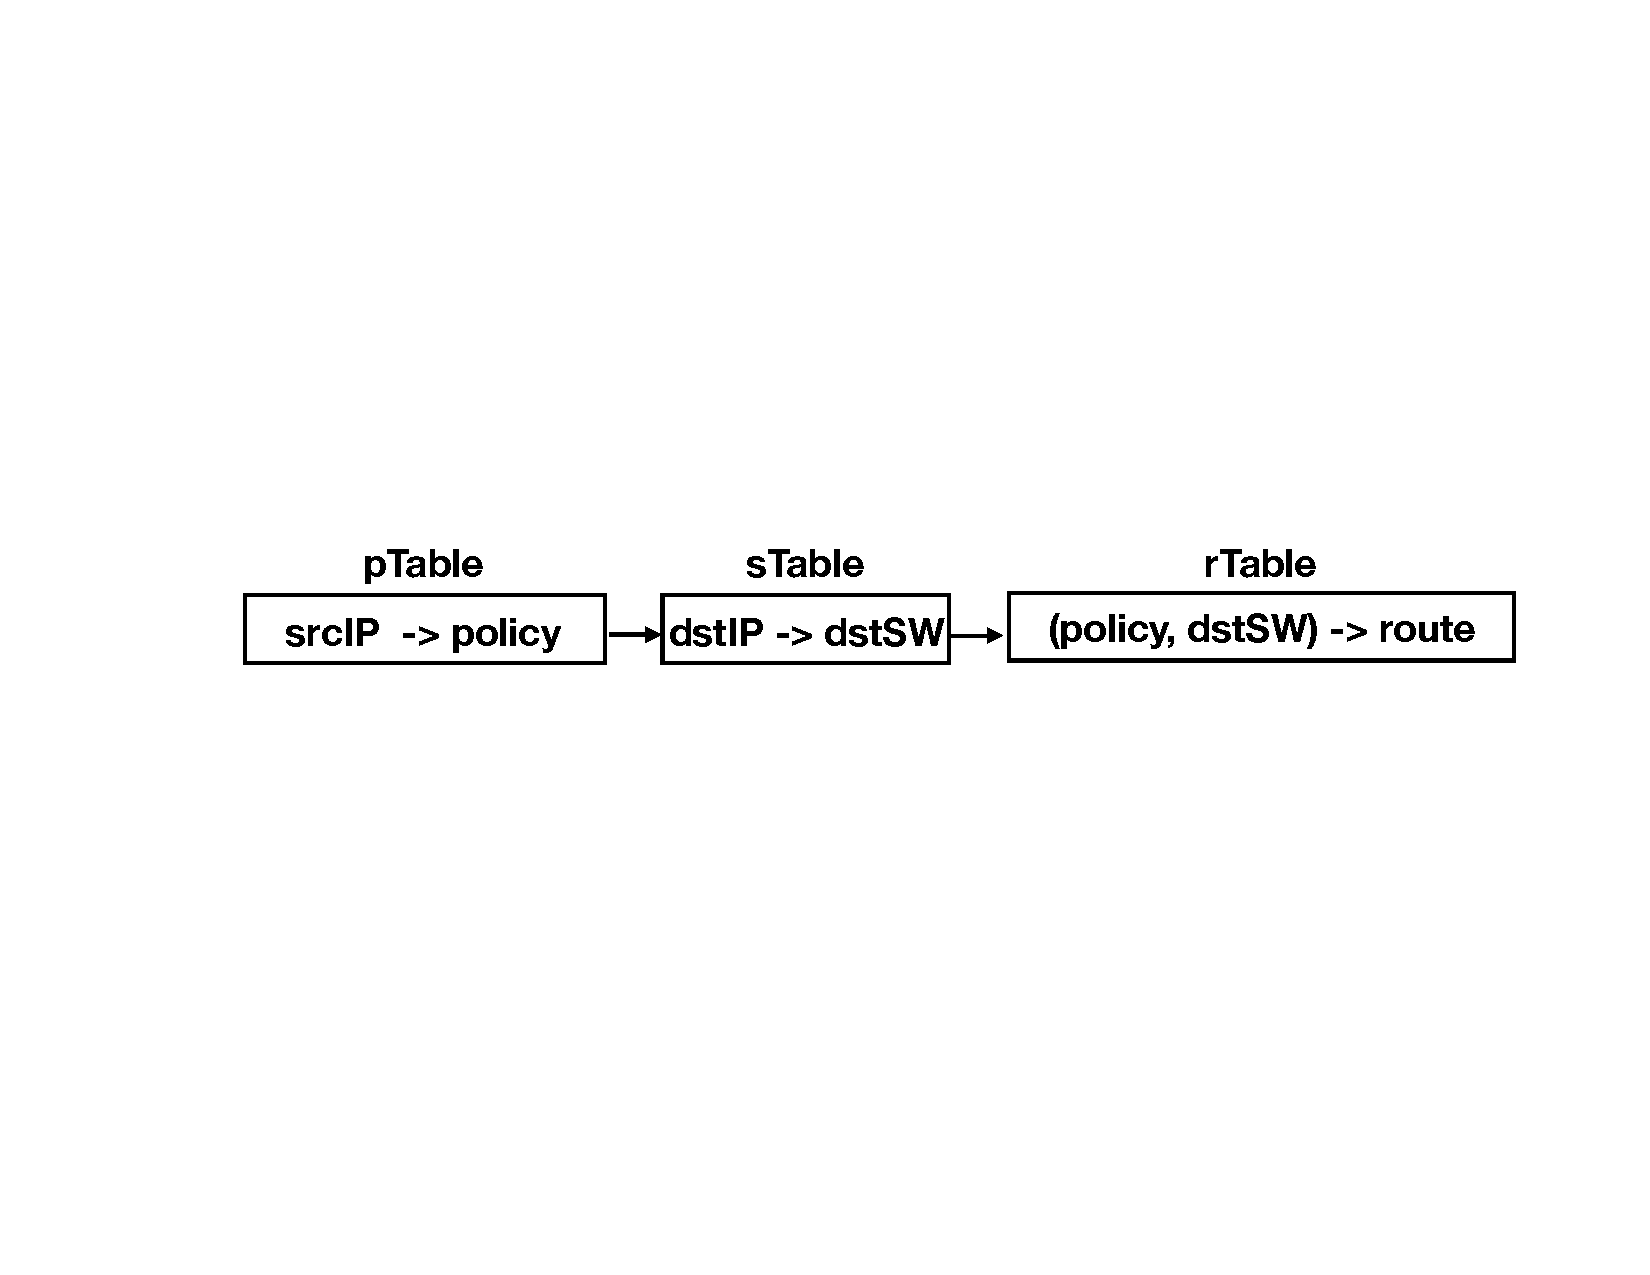
\includegraphics[width=0.8\linewidth]{figures/lp-65.pdf}
\centering
% \vspace{-3mm}
\caption{\small \texttt{SimpleRoute}转换后的三张流表。每张表的结构 $a \rightarrow b$ 表示流表的匹配字段为 $a$以及数据包匹配后可以设置$b$的值。}
\label{fig:srp}
\end{figure}

但是,为了满足OpenFlow交换机的硬件条件(即有限的流表数量),需要在流水线中合并一些表。例如,如果表的数量限制为2,那么\emph{sTable}和\emph{rTable}可以合并为一个表,其匹配项为\emph{dstIP} 和\emph{policy}。我们将此过程称为流水线设计(即决定应合并哪些表)。具体地说,我们将初始流水线称为软件流水线,最终通过合并生成的流水线称为硬件流水线,因为它满足硬件条件的约束。

针对多个具有不同目标和约束条件的流水线设计策略,我们选择减少总流规则数量作为流水线设计的目标以及流表数量作为约束。例如,对于简单路由程序生成的三张流表,在最多允许两个流表的约束下,如果\emph{pTable}和\emph{sTable} 的流规则数量均为1000,\emph{rTable}的流规则数为900,则优先选择合并\emph{sTable}和\emph{rtable}(其流规则总数为1000+1000*900)而不是合并\emph{pTable}和\emph{sTable}(其流规则总数为1000*1000+900)。我们可以看到第二种设计是最优的。这里我们不考虑表合并算法或相应的流规则压缩算法,因为它们已经得到了很好的研究~\cite{ge2015h,gupta2001algorithms}。

\subsection{解决流水线设计中循环问题的研究动机}
为了具有高灵活性,我们应该减少编程模型中的约束。然而,现有的相关工作~\cite{snap,sivaraman2016packet}不能在它们的语言中支持循环。循环的实用性将在如下循环程序(\texttt{SimpleLoop})中说明。

\begin{small}
\begin{verbatim}
L1: def onPacket(pkt):
L2:     p = None; u = Max; ports = allPorts(pkt.dstIP)
L3:     for tp, tu in ports:
L4:         if u > tu:
L5:             u = tu
L6:             p = tp
\end{verbatim}
\end{small}

\texttt{SimpleLoop}首先初始化一个端口 (\emph{p})及其利用率(\emph{u}),并选择一组潜在端口(L2)。然后它遍历所有可能的端口(L3到L6),并比较它们的端口利用率,选择利用率最低的端口。虽然该程序可以通过提供一个用于端口选择的API实现,而不使用循环,但是API会给端口选择策略添加约束。程序员应该有足够的灵活性,并用高级语言(即L4到L6)实现自定义的端口选择策略。 

%As existing SDN datapaths (\eg,~\cite{ofdpa}) do not support loops, we explore methods of implementing loops in the designed hardware pipeline.
由于现有的SDN数据通路(例如~\cite{OF-DPA})不支持循环,因此为了在底层数据通路上实现需要对循环进行转换。有两种可能的转换方法:
%how to achieve the pipeline design for the SDN program with a loop is the issue as the designed hardware pipeline should be put to the datapath. To resolve the issue, there are some potential approaches. 

第一种方法是黑盒方法,它将整个循环视为单个语句。\texttt{SimpleLoop}中的循环可以看作是一个单独语句,进而可以视为单个流表。其中的匹配项包括\emph{p}, \emph{u}, 和 \emph{dstIP}。这种方法的问题是:1. 不能利用数据通路中的多流表流水线结构;2. 由于循环中迭代之间的数据依赖性,流表合并后相应的流表内容很难生成。

第二种方法是应用编译器领域中的循环展开技术。通过循环索引(即\codeword{i}的值)可以对循环进行展开。例如,\texttt{SimpleLoop}的循环可以转换为:

(我们首先把 \codeword{for tp, tu in ports} 转换为 \codeword{for i in len(ports)}。)

\begin{small}
\begin{verbatim}
L1: def onPacket(pkt):
L2:     ... 
L3:     i = 0
L4:     ... #the loop body
L5:     i = 1
L6:     ... #the loop body
L7:     ... #i from 2 to len(ports) - 1
\end{verbatim}
\end{small}

该做法的优点是转换后的程序可以应用于流水线设计。但其局限性是:1. 循环展开技术只能处理静态循环条件(例如显式的迭代次数)。而循环条件可以是动态的(例如 \codeword{while pkt.vlan is None}),所以这种方法是受限的;2. 即使循环可以转换为顺序语句,但长的语句序列可能会降低流水线设计的性能。

因此我们提出RSP(Repeated Software Pipeline)的循环编译转换方法。该方法支持动态循环条件并计算循环的最佳流水线时显示出更高的效率。




\section{重复软件流水线(RSP)转换}
\label{sec:model}

在本节中,我们将首先描述在流水线设计中引入循环之后的一些关键概念,然后再根据这些概念导出RSP转换。
%Then, we will introduce the RSP transformation as motivated by these concepts.
\subsection{关键概念}
\para{流水线}: 由于这里的流水线包括软件流水线和硬件流水线,而软件流水线更贴近与对程序的建模,因此我们这里对上一章的流水线模型进行了拓展(即引入输入/输出变量的概念)。流水线$pl$由一系列表$t_1, t_2, ... t_m$组成。每个表$t_i$指定一组变量 $t_i.inputV$ 作为输入变量,另一组变量$t_i.outputV$作为输出变量。(即到达$t_i$的数据包可以匹配$t_i.inputV$ 并将值写入 $t_i.outputV$。)路由操作,例如Drop或Forward(port=i),属于特殊输出变量的实例。当一个数据包$pkt$在没有任何路由操作的情况下通过$t_i$ 后,$pkt$可以跳转到表$t_j$,其中 $i < j$ 保证$pl$中没有循环。我们将一组变量 $pl.inputV$ 称为$pl$ 的输入变量,且$pl.inputV = (\cup_{i = 1, 2, ..., m}t_i.inputV - \cup_{i = 1, 2, ..., m}t_i.outputV)$,又将一组变量 $pl.outputV$称为$pl$ 的输出变量,且$pl.outputV = (\cup_{i = 1, 2, ..., m}t_i.outputV - \cup_{i = 1, 2, ..., m}t_i.inputV)$。具体来说,流水线的输入、输出变量是指从外部访问流水线的变量(即它们可以在流水线之前设置,在流水线之后读取)。如果表 $t$有一个输入变量是 $v_a$,则变量 $v_a$是$t$的隐藏输出变量,这是因为如果$t$中的一条规则匹配了$v_a$的一个值,则该规则也必然输出相同的$v_a$值。 

\para{静态单赋值}:给定流水线$pl$,$pl$的静态单赋值(SSA)形式意味着$pl$中的每个变量只能赋值一次。SSA的一个例子可以在图~\ref{fig:pipelines}中看到。从现在起,我们假设每个流水线都是具有SSA形式的。

\para{循环条件和循环体}: 给定高级SDN程序中的循环,循环条件是判断数据包是否进入循环的控制语句。循环体是应用于数据包的重复过程。为了简单但不丢失普遍性,我们考虑拥有布尔条件为循环条件、重复代码块为循环体的\emph{while-loop}。如果循环次数是执行时才确定的,则表示该循环条件是动态的。

\subsection{重复软件流水线(RSP)转换}

给定高级SDN程序中一个循环,RSP转换将执行以下操作:1. 提取循环条件和循环体,并将它们链接在一起以生成新的语句集;2. 计算新语句集的软件流水线(每个语句都可以看作一个流表);3. 连接软件流水线的多个副本并生成RSP。举例说明,如果循环条件是\codeword{while i < len(pkt.segmentList)}循环体是\codeword{test = True if check(pkt.srcAddr, pkt.segmentList[i++]) else False},则软件流水线是 $(i, segmentList) \rightarrow None$, $(srcAddr, segmentList, i) \rightarrow (i, test)$。第一个表用于检查是移动到下一次循环过程还是中断循环。RSP则是将该软件流水线的多个拷贝连接在一起。以下是RSP的定义:

\begin{definition}
给定有相同的布局和流规则的$n$个流水线(表示为$pl_1$, $pl_2$, ... $pl_n$),我们用$pl^n$表示$n$个顺序连接$pl_1$, $pl_2$, ... $pl_n$构成的RSP,并称为n-RSP。
\end{definition}

给定一个$pl^n$,当一个数据包$pkt$ 在没有任何路由操作(如Drop或Forward(port=i))的情况下通过$pl_i$时,$pkt$将到达$pl_{i+1}$,其中$1 \leq i < n$。RSP及其SSA形式的示例如图~\ref{fig:pipelines}所示。

\begin{figure}[!htbp]
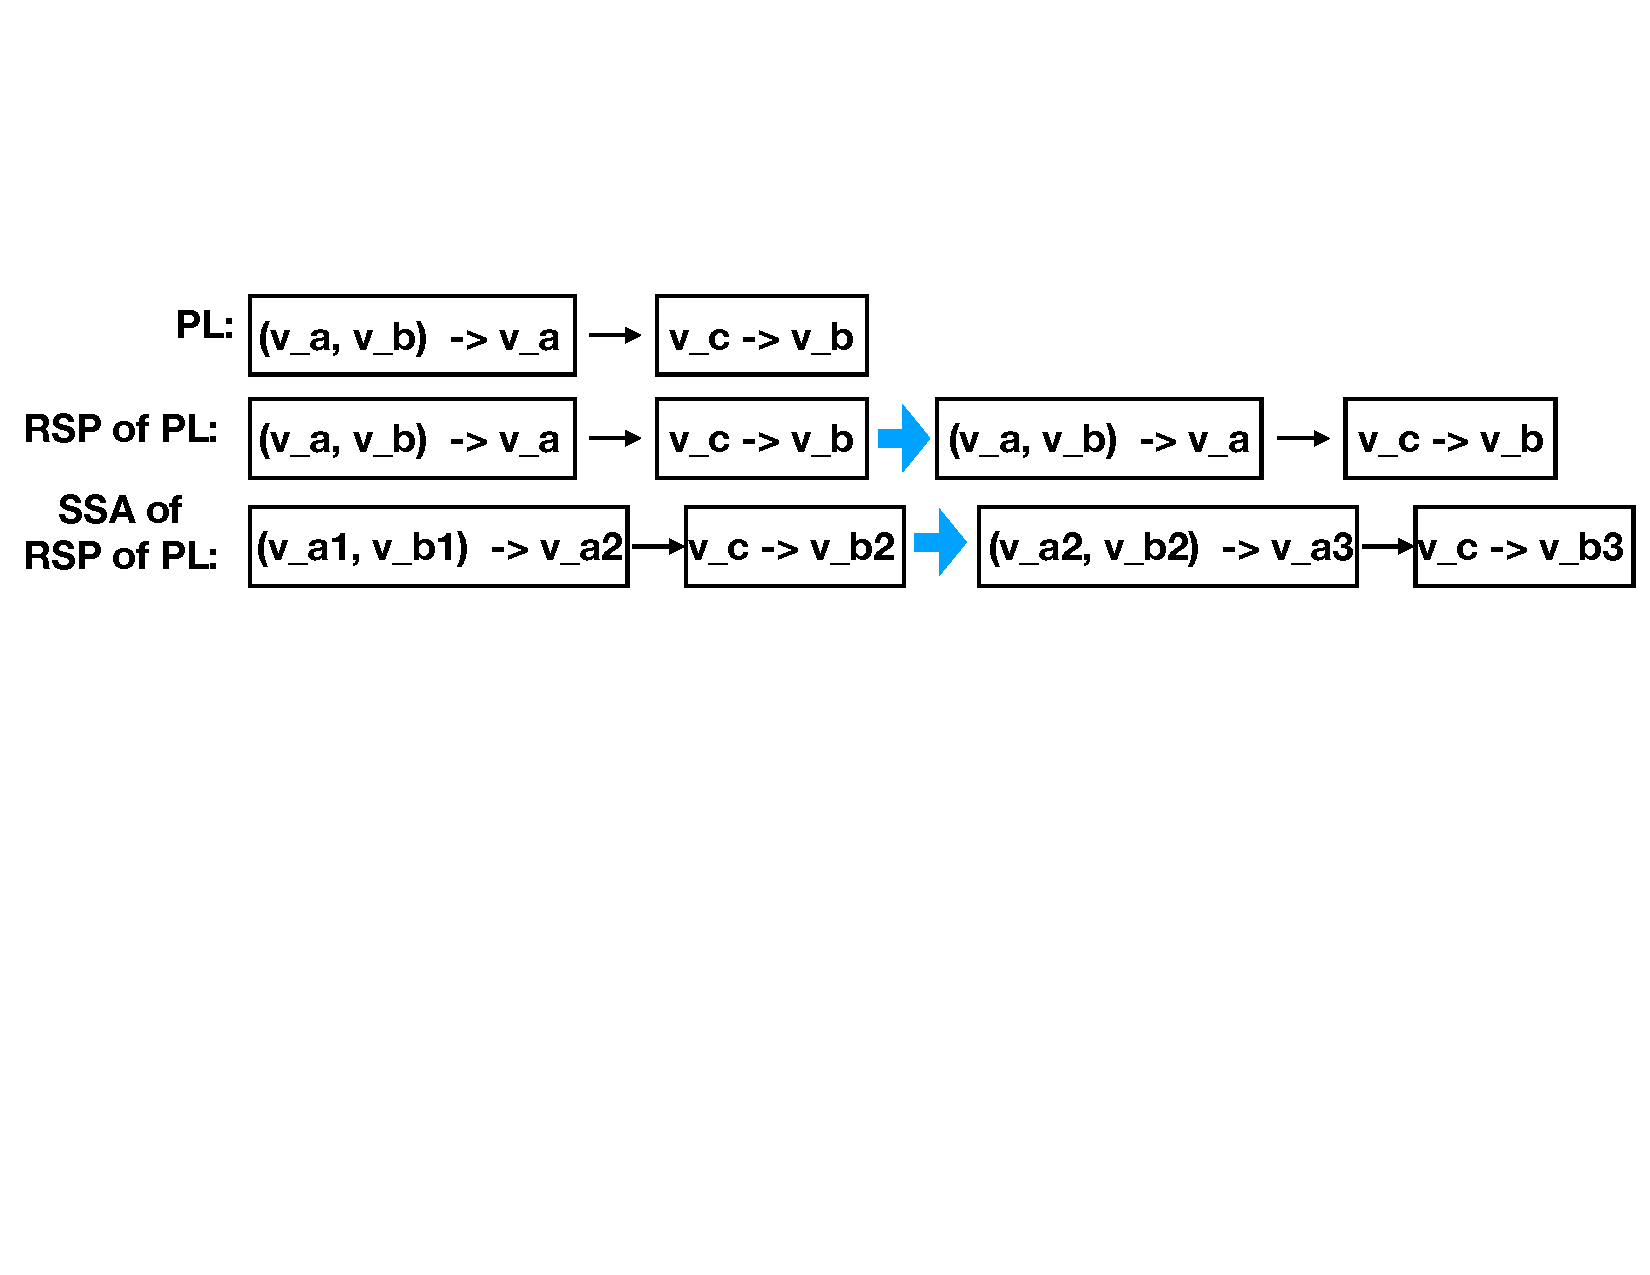
\includegraphics[width=0.93\linewidth]{figures/lp-66.pdf}
\centering
% \vspace{-3mm}
\caption{\small 流水线$PL$, $PL$的2-RSP形式($PL_{RSP}$),SSA形式($SSA(PL_{RSP})$)。}
\label{fig:pipelines}
\end{figure}

对于给定的循环及其对应的RSP,如果一个数据包$pkt$通过重复$n$次进入该循环,然后生成一个输出,那么该输出于与$pkt$进入n-RSP的输出相同。直观理解是(考虑循环把$i$从$0$迭代到$n$ ),对于重复软件流水线中的每个软件流水线,虽然它与其它的没有区别,但是每个流水线都会读一个上一个流水线更新过$i$的值以及增加$i$的值 。因此,到达不同流水线的数据包可以应用不同的规则,然后通过$n$个相同的流水线,它可以得到与循环的$n$ 次迭代过程后相同的输出。

在介绍了RSP之后,我们将其应用到流水线设计中。在下一节中,我们将对基于RSP的流水线设计进行分析,以说明流水线设计可以有效地完成(即RSP的有效性)并支持动态循环条件。



\section{流水线设计以及RSP分析}
\label{sec:analysis}

在这一节中,我们首先分析了流水线的最优设计。然后,我们对RSP进行了分析,以证明其高效和有效性。

\subsection{最优化流水线设计}
我们根据流水线的数据流图将流水线设计归类为一个分割问题。

\para{流水线数据流图}: 给定一个流水线$pl$,我们称 $DFG(pl)$ 是这个流水线$pl$ 的数据流图(DFG),它是一个有向无环图$(V, E)$。其中点$v \in V$表示流水线$pl$ 中的一个变量,并且如果存在$pl$中的一个表$t_i$,它的$t_i.inputV = \{v_{i1}^i, v_{i2}^i, ... v_{i|t_i.inputV|}^i\}$且$t_i.outputV = \{v_{i1}^o, v_{i2}^o, ... v_{i|t_i.outputV|}^o\}$,则有$|t_i.inputV| * |t_i.outputV|$ 条有向边 $v_{i1}^i \to v_{i1}^o$, $v_{i2}^i \to v_{i1}^o$, ..., $v_{i|t_i.inputV|}^i \to v_{i|t_i.outputV|}^o$在$E$中。图~\ref{fig:pipelines}中SSA形式的流水线的DFG在图~\ref{fig:dfg}中所示。

\para{源节点选择}: 首先从DFG中的源节点(即入度为零的节点)中选出一个子集并放入$S$,如果DFG中的一个节点$v$的所有父节点都在$S$中,则可以将$v$添加到$S$中。一个选择可以包含多次添加过程。选择完成后,从原始DFG中移除$S$(即$S$从DFG中分割),然后$S$可以被视为一张流表$t$。在$S$中且没有任何父节点的节点被添加到$t.inputV$,在$S$中且没有任何子节点的节点被添加到$t.outputV$。源节点选择的示例如图~\ref{fig:dfg}所示。其中 $v_{a2}$可以添加到$S1$,但$v_{a3}$ 不能(即使将$v_{a2}$添加到$S1$之后),因为它的一些父节点不在$S1$中。通过将$v_{b2}$和 $v_{b3}$添加到$S2$,当前选择可以有三个表(如图~\ref{fig:dfg}中的红点线所示): $(v_{a1}, v_{b1}) \rightarrow v_{a2}$, $v_c \rightarrow (v_{b2}, v_{b3})$, 以及 $(v_{a2}, v_{b2}) \rightarrow v_{b3}$ 。

\begin{figure}[!htbp]
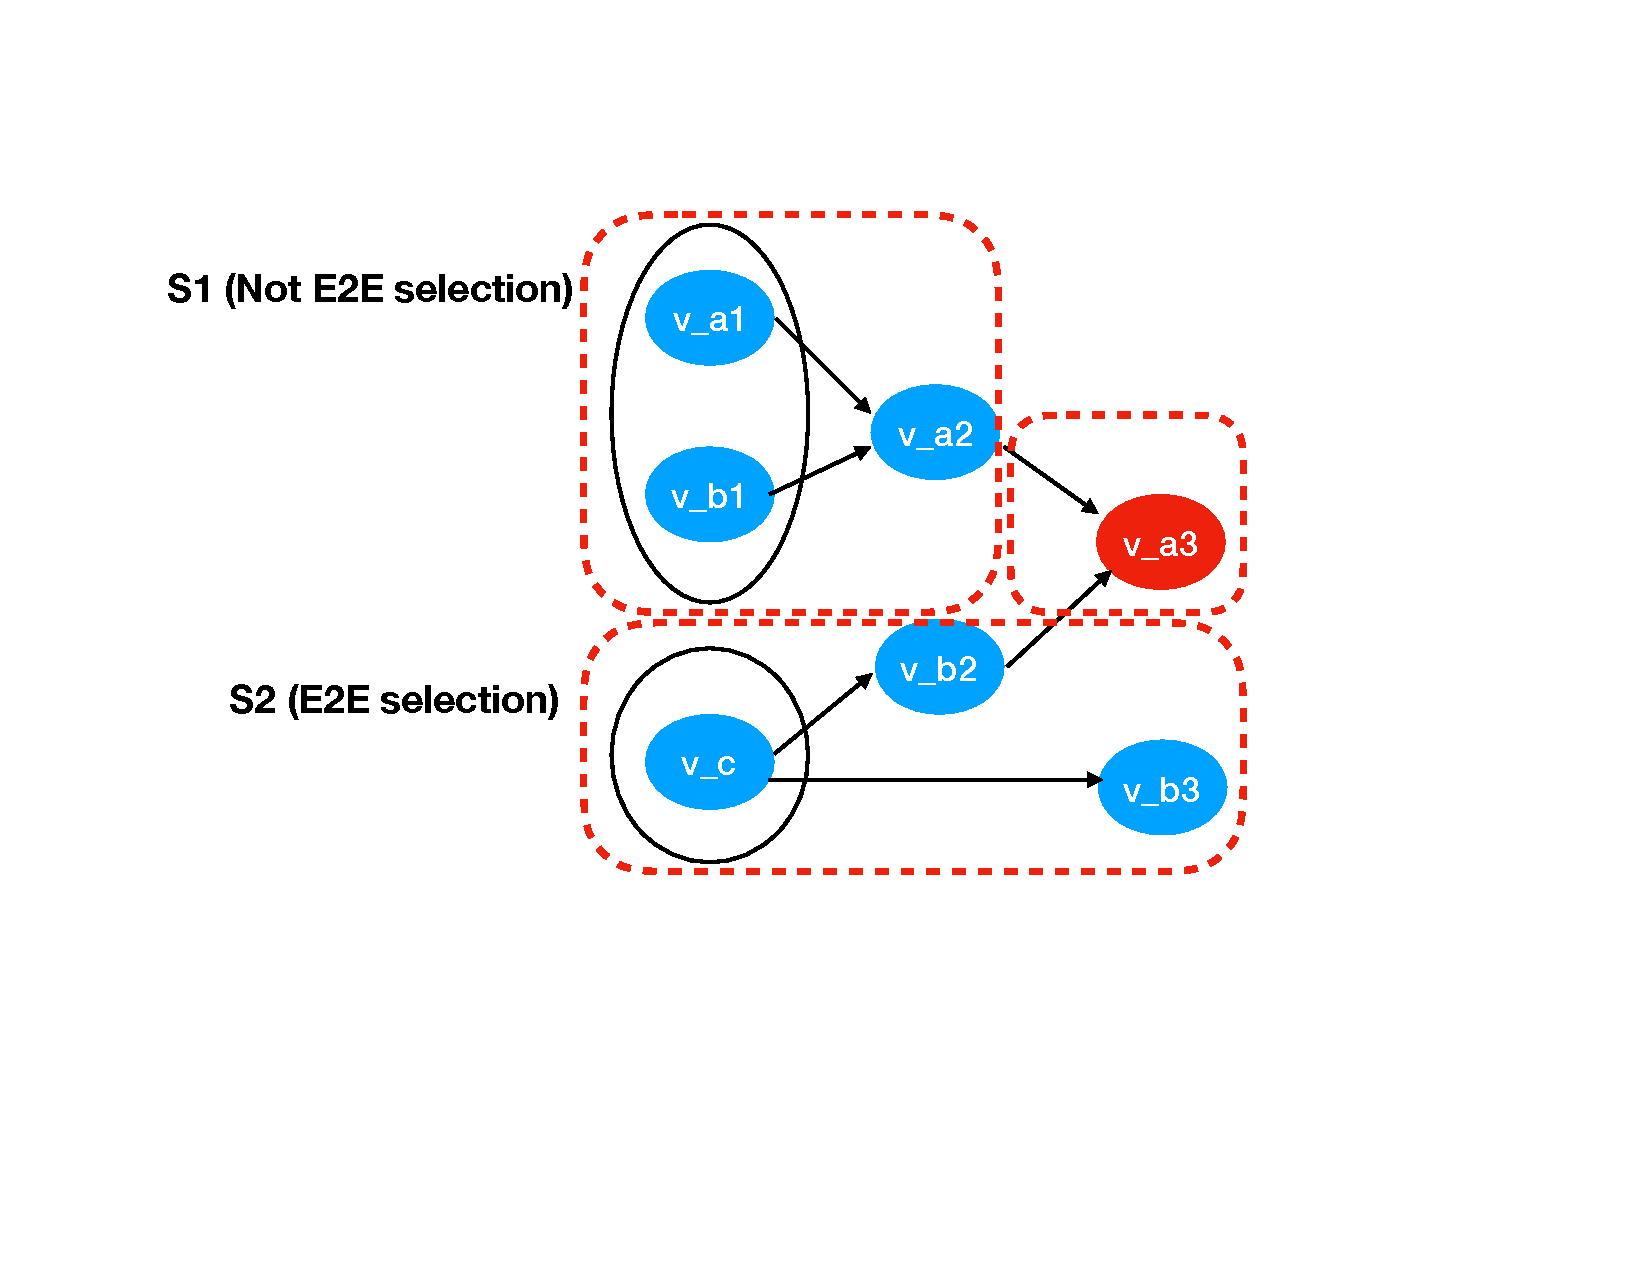
\includegraphics[width=0.6\linewidth]{figures/lp-67.pdf}
\centering
\vspace{-3mm}
\caption{\small 流水线的DFG和源节点选择。}
\label{fig:dfg}
\end{figure}

流水线设计可以视为流水线DFG中的多次源节点选择。如果流水线设计对底层数据通路的约束为最多$k$个流表,那么最多会有$k-1$ 源节点选择。

\para{最优流水线设计的贪婪性}: 如果流水线设计是最优的,则意味着生成的流水线具有最少的流规则数量。在这种情况下,选择的每一步都应该是``贪婪的''。即,如果$v$可以添加到$S$中,则它应该被添加。我们将此属性表示为贪婪选择性质。例如,在图~\ref{fig:dfg}中,为了获得最佳的流水线,应该将$v_{b3}$添加到$S2$中,否则还有另一个表:$v_c \rightarrow v_{b3}$。一个简单理解则是,如果有两个流表$t_1$和$t_2$,以及$t_2.inputV \subseteq (t_1.inputV \cup t_1.outputV)$,那么将$t_2$ 合并到$t_1$中不会添加额外的流规则。这意味着在优化的流水线设计中,$t_2$应该合并到$t_1$中,以减少对应的数据包需要的处理步骤的数量,降低数据包的处理时延。

\subsection{重复软件流水线的分析}
基于最优流水线设计的贪婪特性,我们论证流水线设计在RSP上执行的有效性和效率情况(通过分析)。我们首先给出流水线优化设计的目标。

\para{最优流水线设计的目标}: 在硬件限制下(即最多可以实现$k$个表),在$pl^n$($k < n$)上计算具有最小流表规则数量的流水线。由于流水线深度影响通过流水线的数据包的时延,如果有满足约束的两条流水线具有相同数量的流规则,优先选择表数较少的流水线。

\para{复杂度}: 由于流水线设计的复杂度取决于DFG中的节点数量,因此$n$很大的$pl^n$的流水线设计是一个非常复杂的过程。然而,我们发现并证明复杂度依赖于$k$,而不是$n$(在$k < n$下)。

我们首先提出三个概念:单一输出流水线、E2E选择和全输出表。

\para{单一输出流水线}: 一个流水线$pl$,其中$pl$的输出变量只出现在$pl$的最后一个表中。我们将这种流水线表示为单一输出流水线(Single-output Pipeline,SO-PL)。SO-PL的例子在图~\ref{fig:sopl}中所示。
%The example of SO-PL is shown in Figure~\ref{fig:sopl} where $v_d$ is the only output variable.
%
\begin{figure}[!htbp]
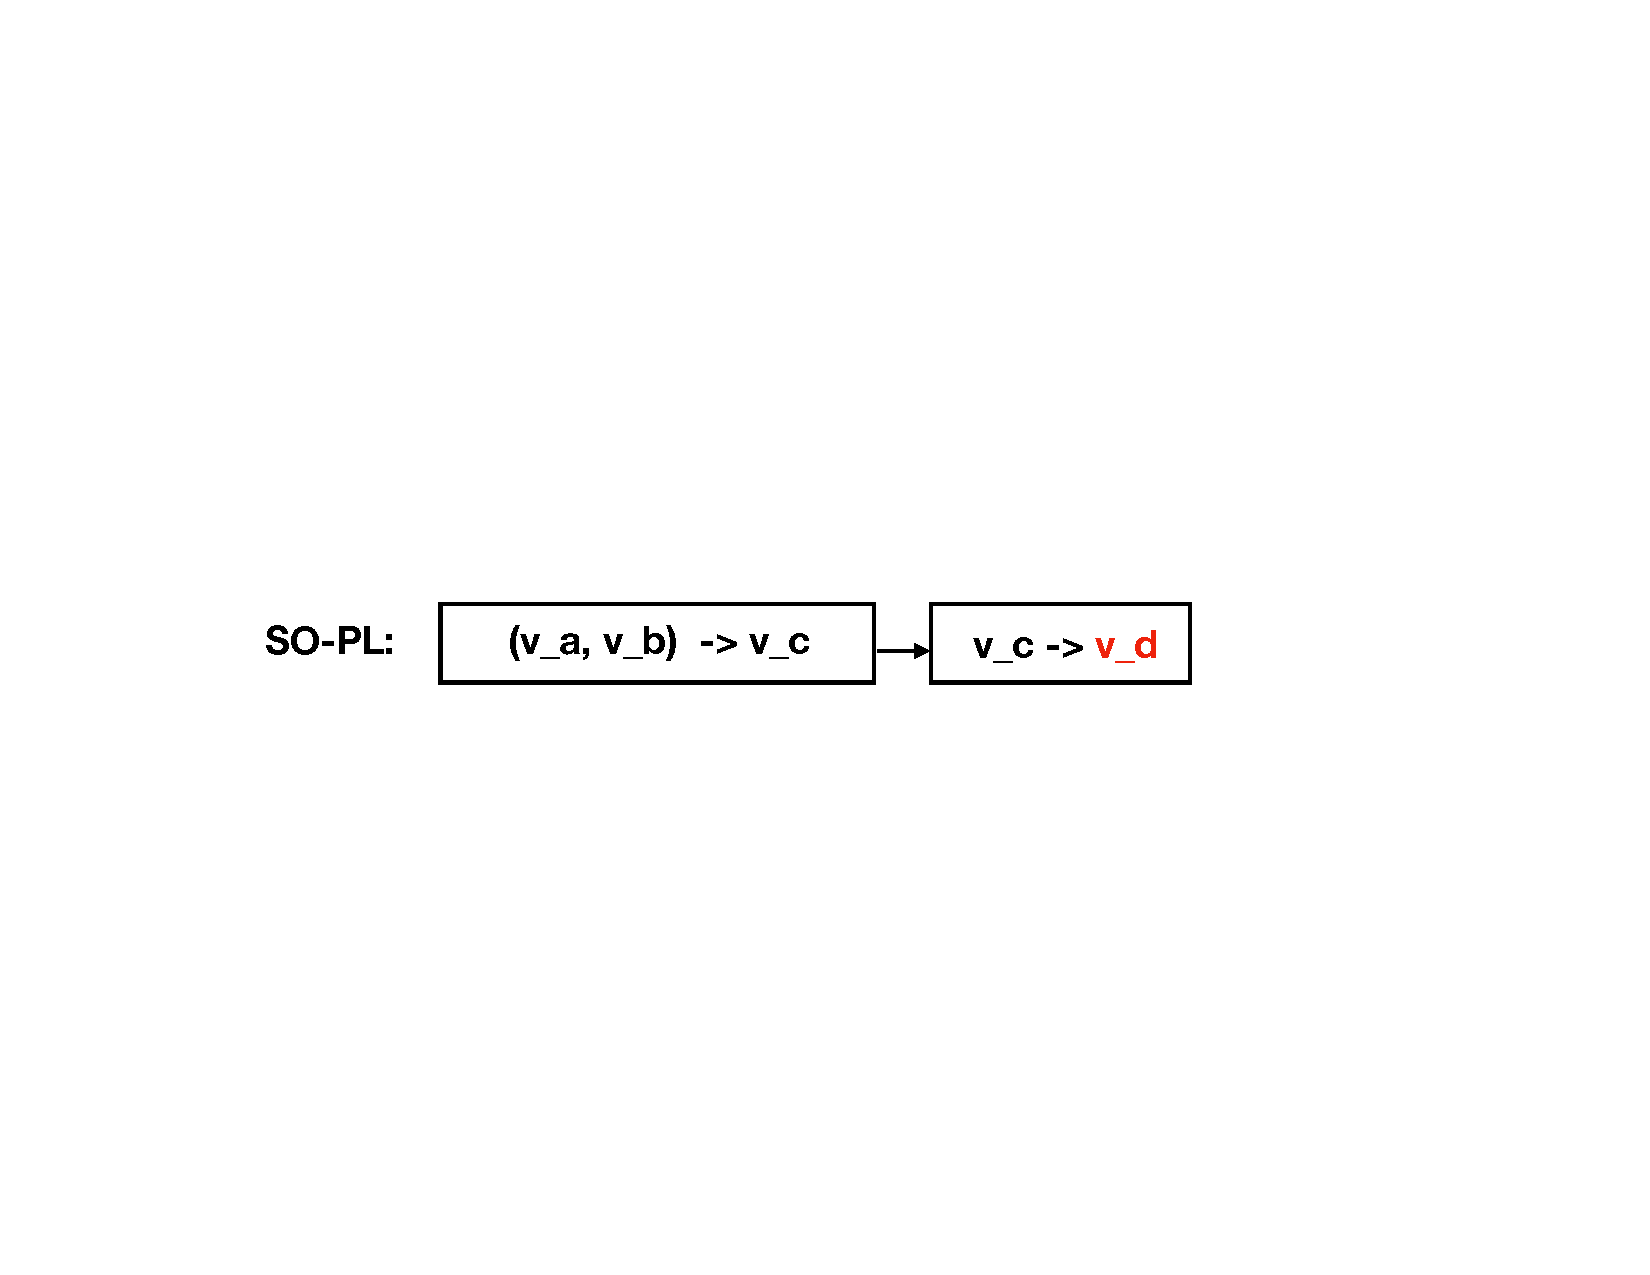
\includegraphics[width=0.8\linewidth]{figures/lp-68.pdf}
\centering
\caption{\small SO-PL的示例,其中$v_d$为流水线唯一输出变量。}
\label{fig:sopl}
\end{figure}

\para{E2E选择}: 如果DFG上的源节点选择出的节点集合(包含所有源节点的真子集,而非全部源节点)中至少有一个DFG中的汇节点$v$,则该选择称为E2E(End-to-end)选择。E2E选择的示例如图~\ref{fig:dfg}所示。其中$S1$不是E2E选择,因为$v_{a3}$也依赖于$v_{b2}$。但是$S2$是E2E,因为$v_{b3}$只依赖于$v_c$。

根据E2E选择的定义,我们发现SO-PL中没有E2E选择。对于至少选择了一个汇顶点$v$的选择,$v$的祖先应该是所有的源顶点(而不是一个真子集)。

\para{全输出表}: 给定$pl^n$,如果一个表$t_x$的输出变量包含流水线$pl_i$的所有输入变量,则$t_x$是$pl^n$的全输出表。根据贪心性质,如果是最优流水线设计,则所有剩余的表都应合并到$t_x$中。如果有多个流水线的输入变量包含在$t_x$的输出变量中,我们将这些流水线的最小索引定义为 $MinIndexPL(t_x)$。考虑图~\ref{fig:pipelines}中SSA格式流水线($SSA(PL_{RSP}$)),考虑一个流表$t_y$,其输出变量为$v_{a2}, v_{b2}, v_c$,则$t_y$是$SSA(PL_{RSP}$的全输出表。当$SSA(PL_{RSP}$的第二条流水线合并到$t_y$后,其第三条流水线(图中未显示)也合并到$t_y$中。在这种情况下,$MinIndexPL(t_y)$仍然是2,即是第二条流水线的索引。

%there is at least one sink vertex $v$ in the graph with the constraint: $\forall$ source vertices that have paths to $v$ in the graph, these source vertices are in the partitioned source vertices of $C_p$.

在流水线设计中,我们对全输出表的存在性得出以下定理。

\begin{theorem}
\label{lp-prop1}
存在性:如果$DFG(pl_i)$ $\forall i \in 1, 2, ... n$中没有E2E选择,那么通过流水线设计将$pl^n$合并到$k$个表($k < n$),合并的$k$个表中至少存在一个全输出表$t_x$。
\end{theorem}

\begin{proof}
我们用反证法,即假设合并的$k$个表中不存在这样的$t_x$。

基于这个假设,我们给出了一个流水线设计,它将$pl^n$合并到最少数量的表中,如图~\ref{fig:proof}所示。对于第一个流水线 $pl_1$,我们选择 $pl_1$的输入变量的真子集来得到表$t_1$。(我们避免使用全部输入变量,因为这样会得到一个$t_x$)。由于没有E2E选择,$t_1$的输出变量不能包括$pl_1$的任何输出变量。我们考虑第二个表$t_2$,其中输入变量是剩余DFG中的所有源节点(这与原始源节点不同,因为已经对一组节点进行了分割)。我们发现$t_2$的输出变量不能是$pl_2$的全部输入变量,因为不能有$t_x$。同样地,$t_3$的输出变量不能包含$pl_3$的全部输入变量。

我们发现这种流水线设计给出的表的最小数目是$n+1$。但是,我们有$n + 1 > k$(它超出了流表数量的限制),因此没有$t_x$的假设是错误的。
\end{proof}


\begin{figure}[!htbp]
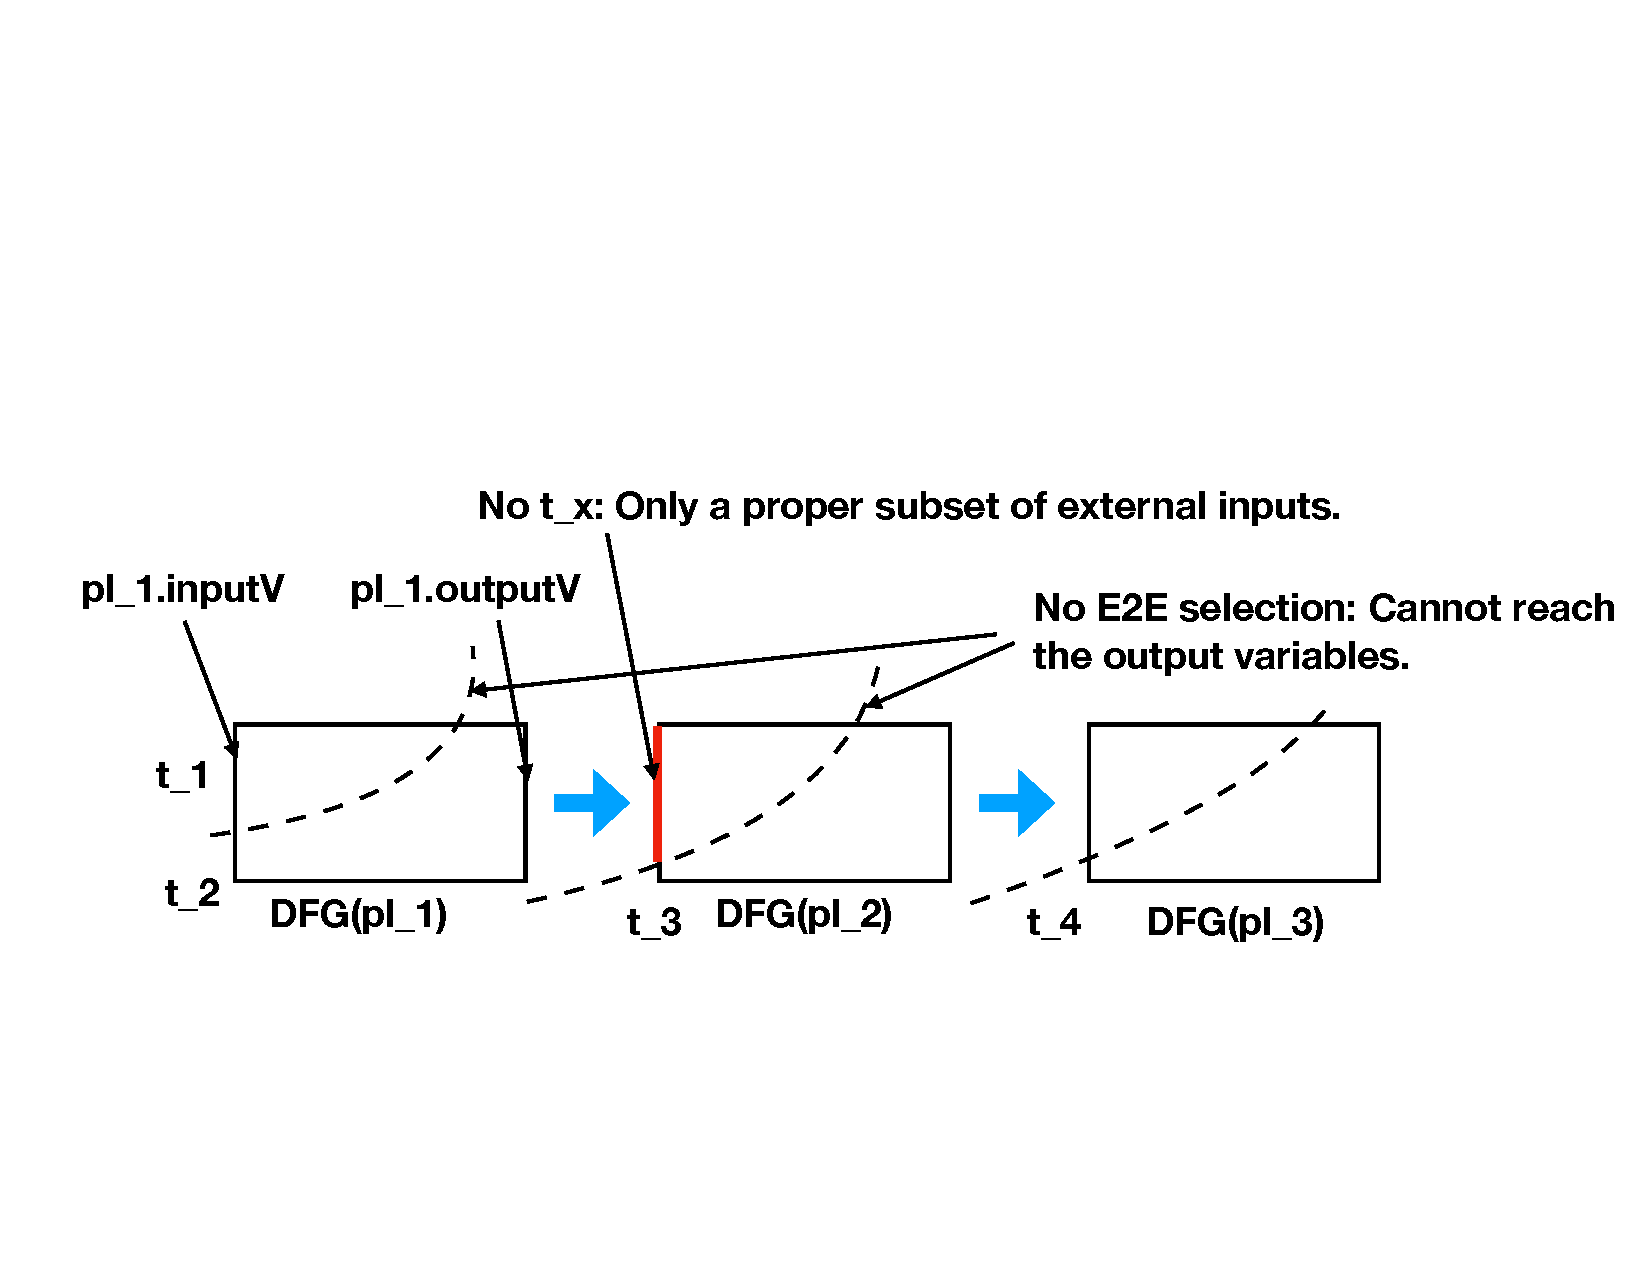
\includegraphics[width=0.9\linewidth]{figures/lp-69.pdf}
\centering
\caption{\small 存在性定理的证明, 图中三个流水线 ($pl_1, pl_2, pl_3$) 在假设下只能被合并到至少四张表 ($t_1, t_2, t_3, t_4$) 。每个方块是一个流水线的DFG.}
\label{fig:proof}
\end{figure}

存在性定理表明,如果我们要将$pl^n$合并到$k < n$的$k$个表中,并且如果$pl^n$的DFG中没有E2E选择,那么合并表中至少存在一个全输出表。由于该定理不涉及流水线设计的最优性,因此可以得到多个全输出表。

基于全输出表存在性的定理,我们给出了考虑最优流水线设计的全输出表的位置定理。

\begin{theorem}
位置:如果$DFG(pl_i)$ $\forall i \in 1, 2, ... n$中没有E2E选择,那么通过最优流水线设计将$pl^n$放到至多$k$个表($k < n$)时,在最多$k$个表合并后,必须只有一个全输出表$t_x$,且$MinIndexPL(t_x) \leq k$。
\end{theorem}

\begin{proof}
如果出现一个全输出表,为了优化流水线设计的需要(即贪婪性质),下面所有的表/流水线都应该合并到全输出表中。因此,只有一个全输出表$t_x$。如果$MinIndexPL(t_x) > k$,则必须将开始的$k$个流水线合并到$k-1$表中,这被存在性定理排除。
\end{proof}

%The positioning proposition says that if we want to have the optimal pipeline design of merging $pl^n$ into $k$ tables where $k < n$, and there is no E2E selection in the dataflow graph of pipelines of $pl^n$, then the full-output table must appear in the first $k$ pipelines, which means \emph{the result of pipeline design with only first $k$ pipelines is the same with the whole $n$ pipelines.}

\para{小结}: 如果每个软件流水线都是$pl^n$中的SO-PL(即没有E2E选择),那么对于把$pl^n$放到至多$k$个表($k < n$)的最优流水线设计,流水线设计应该只考虑前$k$个软件流水线,而不是所有$n$个流水线(根据位置定理的结果,用前$k$个流水线设计的结果和用前$n$个相同),这证明了其高效性,因为流水线设计的复杂程度不随着流水线数量$n$而提高。此外,对于有效性,即使不能在执行之前指定迭代次数,对于要最多合并到$k$个表的情况,也只需要考虑前$k$条流水线的最佳流水线设计。 

给定一个全输出表$t_x$,将后续所有表/流水线合并到$t_x$将增加$t_x$的大小。但是,在数据通路设计中,一个逻辑流表可以映射到多个硬件流表~\cite{rmt},这意味着在实现中逻辑表的大小不是问题。

\para{放宽约束}: SO-PL约束也可以通过以下方式放宽:每个软件流水线的DFG至少有一个汇节点,其祖先为所有源顶点。一个例子是图~\ref{fig:dfg}中的$v_{a3}$,它的祖先是所有的源顶点。我们可以看到,SO-PL是一个特殊情况,其中所有汇节点都将所有源顶点作为祖先。一个简单的证明:我们首先假设$pl^n$可以合并到$k$个表中,而不需要创建一个全输出表,并且$pl^n$的每个软件流水线至少有一个汇节点($v$)其祖先都是源顶点。我们移除合并后$k$个表中输出变量不是$v$的相应流规则(即,其余的流规则都是$v$的)。根据存在性定理,合并后的$k$表不存在,这意味着假设是不正确的。

在放宽后的约束条件下,即循环中至少有一个依赖于所有输入变量的输出变量,大部分循环可以作为我们提出的设计的目标。而对于不符合此要求的循环,我们可以将循环分成多个子循环(通过现有编译器技术),以便每个循环都满足约束。


\section{实验评估}
\label{sec:eval}

在这一部分中,我们从流水线设计的执行时间和生成的流水线的流规则数量两个方面来评估所提出的RSP设计。所有评估都在16GB内存以及3.5 GHz Intel i7处理器上运行,系统为Mac OSX 10.13。

\subsection{执行时间}
\para{实验方法}: 基于最优流水线设计的分析,考虑以下简单的流水线设计算法:给定一个DFG和$k$,递归地在DFG上应用源节点选择$k-1$次来枚举所有可能的硬件流水线。对于RSP和展开技术(unrolling)的比较评估,我们随机生成具有以下条件的DFG:对于RSP,我们变化RSP中的软件流水线数(即循环的迭代次数$n$)和每个流水线DFG中的节点数;对于展开技术,从RSP中生成的图的每一个软件流水线中随机移除几个节点。然后,我们比较流水线设计算法应用在RSP生成的图和展开技术生成的图的执行时间。因为我们没有考虑合并算法,枚举所有可能的流水线的复杂性相当于找到最佳流水线的复杂度。


\para{实验结果}: 结果如图~\ref{fig:eval1-loop}所示。水平轴指定循环的迭代次数($n$)。图~\ref{fig:eval1-loop-a}和图~\ref{fig:eval1-loop-b}之间的不同点是每个软件流水线的DFG中的节点数($m$)(对于展开技术,它是指随机移除节点之前的节点数)。其中图~\ref{fig:eval1-loop-a}中的$m = 10$ ,图~\ref{fig:eval1-loop-b}中的$m = 20$。所有流水线设计都设$k=10$作为流表数量的限制。结果表明,与$k < n$时的展开技术相比,RSP方法缩短了执行时间(大约十倍,当$n = 50$ 且 $m = 10$)。当$n = 10$时,RSP和展开在流水线设计中都考虑10个软件流水线,因此,两种方法的执行时间是相同的。当$n = 100$时,与RSP方法相比,展开的执行时间过长。

\begin{figure}[!htbp]
    %\vspace{-2mm}
    \centering
    \begin{minipage}{0.47\linewidth}
        \centering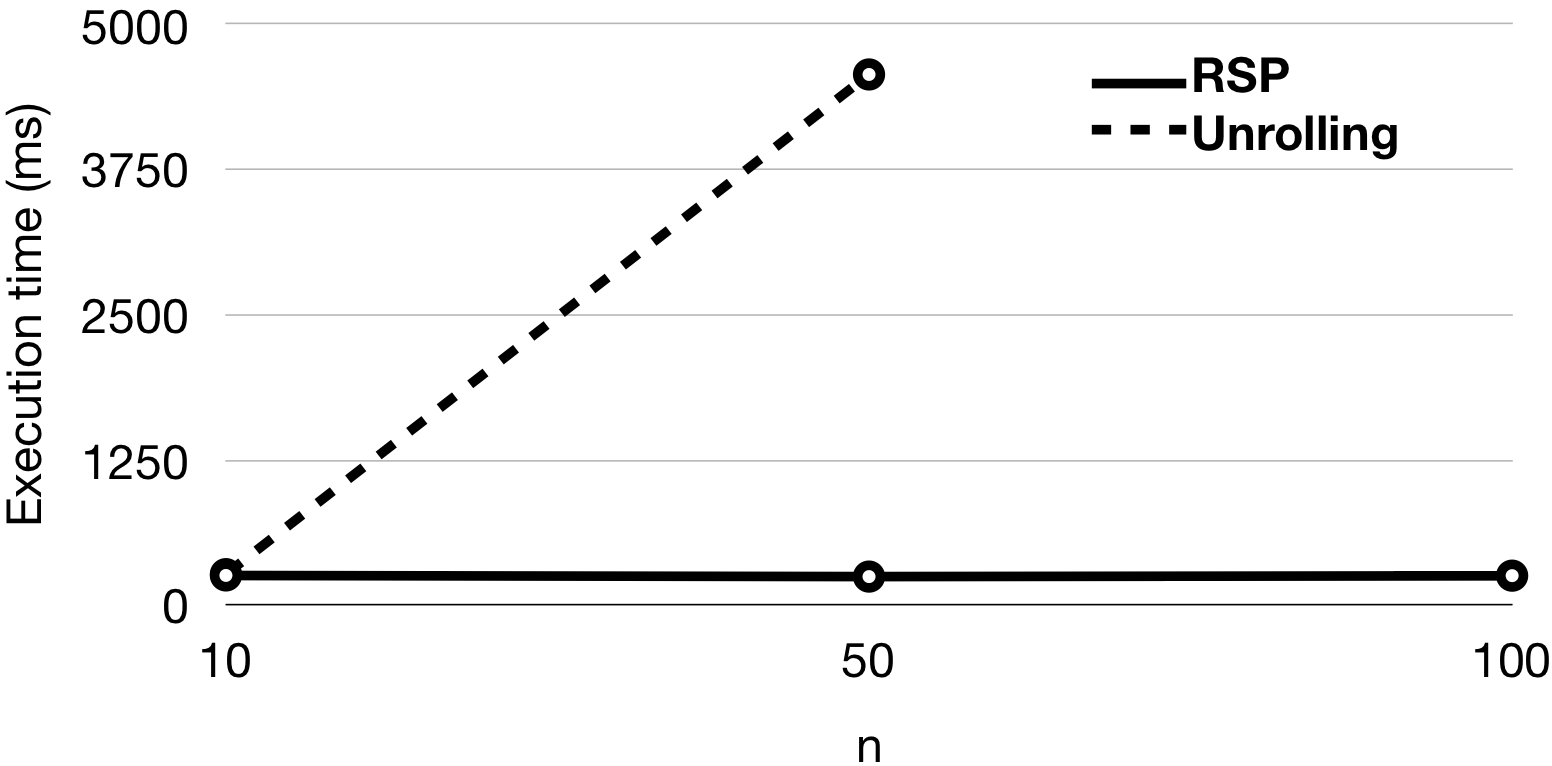
\includegraphics[width=\linewidth]{figures/lp-70.png}
        \caption{\label{fig:eval1-loop-a} \small $m$ = 10.}
    \end{minipage}
    % \hspace{0.03\linewidth}
    \begin{minipage}{0.47\linewidth}
        \centering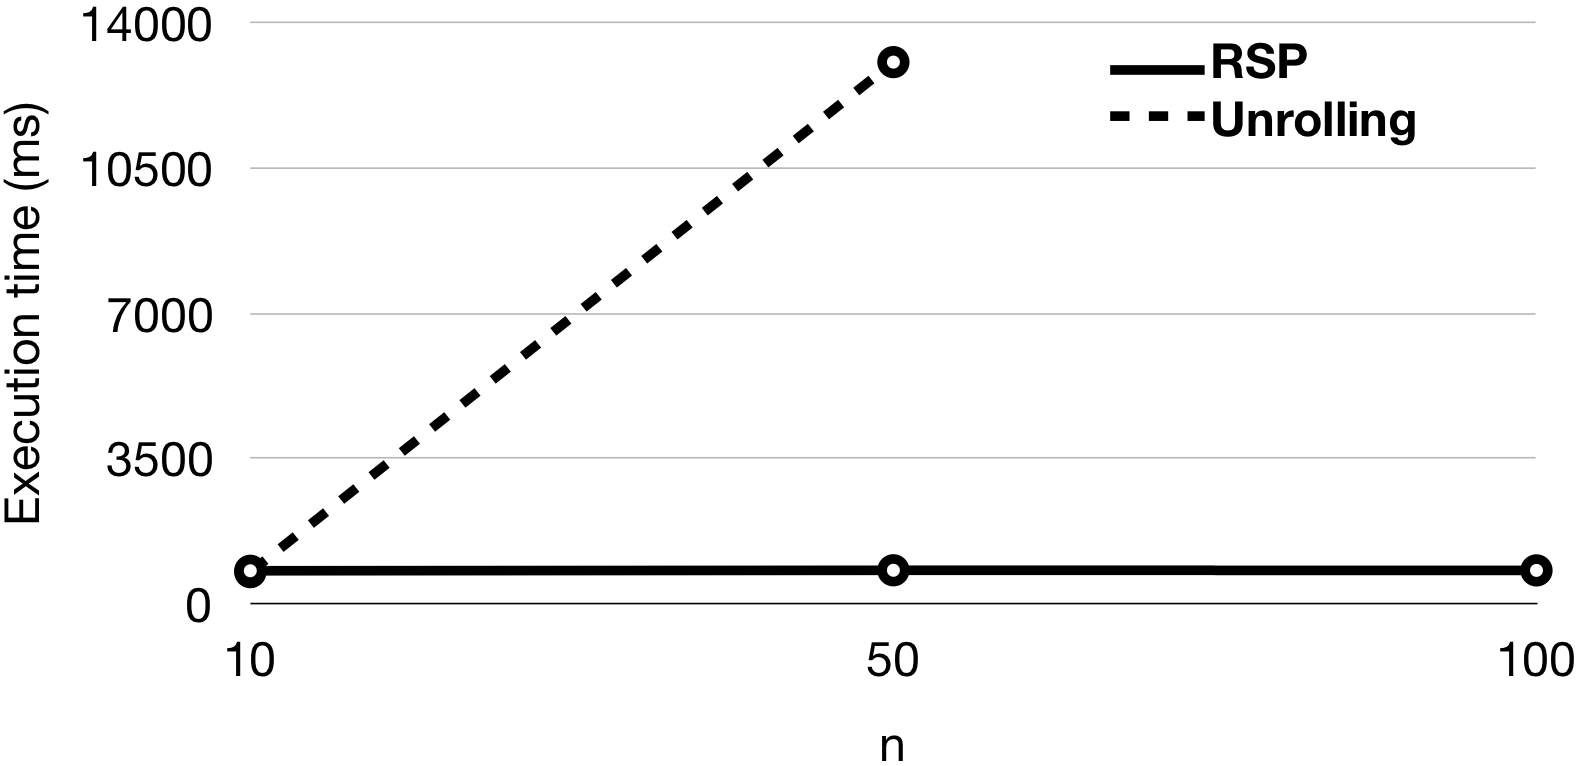
\includegraphics[width=\linewidth]{figures/lp-71.png}
        \caption{\label{fig:eval1-loop-b} \small $m$ = 20.}
    \end{minipage}
    %\caption{\footnotesize{The CDF of job latency local and remote jobs.}}
    \caption{\small 两种方法的执行时间。$n$为迭代次数。$m$为顶点数量。}
    %\vspace{-2mm}
    \label{fig:eval1-loop}
\end{figure}

\subsection{流规则数量}

\para{实验方法}: 为了计算流规则的数量,我们随机给每个变量(即DFG的节点)设置域的大小(即变量的可用值的数量)。具体来说,对于每个软件流水线的DFG中的源节点,我们将其值设置为100到200。对于DFG中的内部节点,我们将值设置为10到20。这是因为对于源节点,它们可能表示数据包字段。与程序中的内部变量相比,数据包字段的值范围应该更大。此外,给定一个流表,流规则数量的计算等于所有输入变量的域大小的乘积。
%For example, if a flow table consists of three input variables and their sizes of domain are 120, 10, 10 respectively, then the number of flow rules of the table is 12000. 
$n$和$m$的定义与上面执行时间的评估时相同。我们比较了RSP设计和黑盒方法(即生成单表)的流规则数量。

\para{实验结果}: 结果见表~\ref{table:eval2}。对于黑盒方法,流规则的数量只取决于所有软件流水线的第一个DFG(等于第一个DFG的所有源节点的域大小的乘积),因此对于不同的$n$,值是相同的。结果表明,与单表设计方法相比,多表设计方法可以显著减少流规则的数量。值得注意的是,对于每个表,RSP方法可能有很多未使用的流规则。例如,可以将\codeword{while i in range(100)}语句视为匹配\emph{i}并包含100条流规则(即\emph{i} = 0, 1, ..., 99)并更改\emph{i}的流表。当该流表作为RSP的第一个流表时,该表有99个未使用的流规则。

\vspace{0.5cm}
\begin{table}[!htbp]
\centering
\scalebox{1.2}{
\begin{tabular}{l|l|l}
\hline
         & n =10, m = 10 & n = 50, m= 10 \\ \hline
Single  & 3898434       & 3898434       \\ \hline
RSP & 61856         & 224098        \\ \hline
\end{tabular}
}
\caption{\small 单表方法和RSP方法下的流规则数。}
\label{table:eval2}
\end{table}

\section{本章小结}

本章针对高级SDN程序中循环结构在可定制结构数据通路的高效实现问题,提出了RSP转换。该方法的可以生成多流表结构,并支持动态循环条件。本文所提出的方法在计算循环的最佳流水线时显示出更高的效率。具体来说,我们证明了对于一类有$n$个循环次数的循环($n$ iteration loop)部署到流表数量有限的多流表流水线中 (设流表的最大数量为$k$),流水线设计只需考虑循环中的前$k$个迭代(我们假设$n > k$)。

